\documentclass[a4paper,12pt]{report}
\usepackage{url}
\usepackage{enumitem}
\usepackage{palatino}
\usepackage[cmex10]{amsmath}
\usepackage{stmaryrd,amssymb}
\usepackage{graphicx}
\usepackage{amsfonts}
\usepackage{rotating}
\usepackage{listings}
\usepackage{xcolor}
\usepackage{url,boxedminipage,listings}
\usepackage{booktabs}
\usepackage{rotating}
\usepackage{array}
\usepackage{color,url,varioref,xcolor}
\usepackage{alltt,epsfig,comment}
\usepackage{supertabular,fancyhdr}
\usepackage{multirow}
\usepackage{url}
\usepackage{xspace}
\usepackage{dsfont}
\usepackage[english]{babel}
\usepackage{todonotes}

\usepackage{pdfpages}
\usepackage[font={footnotesize,sl}, labelfont=bf] {caption}

\usepackage{tikz}
\usetikzlibrary{arrows}
\usetikzlibrary{automata}
\usetikzlibrary{positioning}
\usetikzlibrary{er}

% HAS TO BE LAST PACKAGE:
\usepackage[pdftex,bookmarks=true,pageanchor=false]{hyperref}



% Eiffel Code Stuff
\lstset{language=OOSC2Eiffel,basicstyle=\ttfamily\small}
\definecolor{codebg}{rgb}{0.95,0.95,0.95}
\setlength{\headheight}{28pt}

% Inline Eiffel Code
\let\e\lstinline
% Eiffel Identifiers or expressions
\newcommand{\eid}[1]{\textsl{{\color[HTML]{000000} #1}}}
% Eiffel Class names
%\newcommand{\ecl}[1]{\textsl{{\color[HTML]{3333FF} #1}}}
\newcommand{\ecl}[1]{\textsl{{\color[HTML]{000000} #1}}}
% Eiffel Keywords
%\newcommand{\ekey}[1]{\textbf{{\color[HTML]{333399} #1}}}
\newcommand{\ekey}[1]{\textbf{{\color[HTML]{000000} #1}}}

\newcommand{\distance}[2]{\ensuremath{#1\leftrightarrow#2}}

\newcommand{\blankpage}{
\newpage
\thispagestyle{empty}
\mbox{}
\newpage
}


\title {ABEL Documentation}
\author {
	\textbf{Student:} Roman Schmocker \\
	\textbf{Supervisor:} Marco Piccioni and Bertrand Meyer  
}


\begin{document}

\pagenumbering{roman}
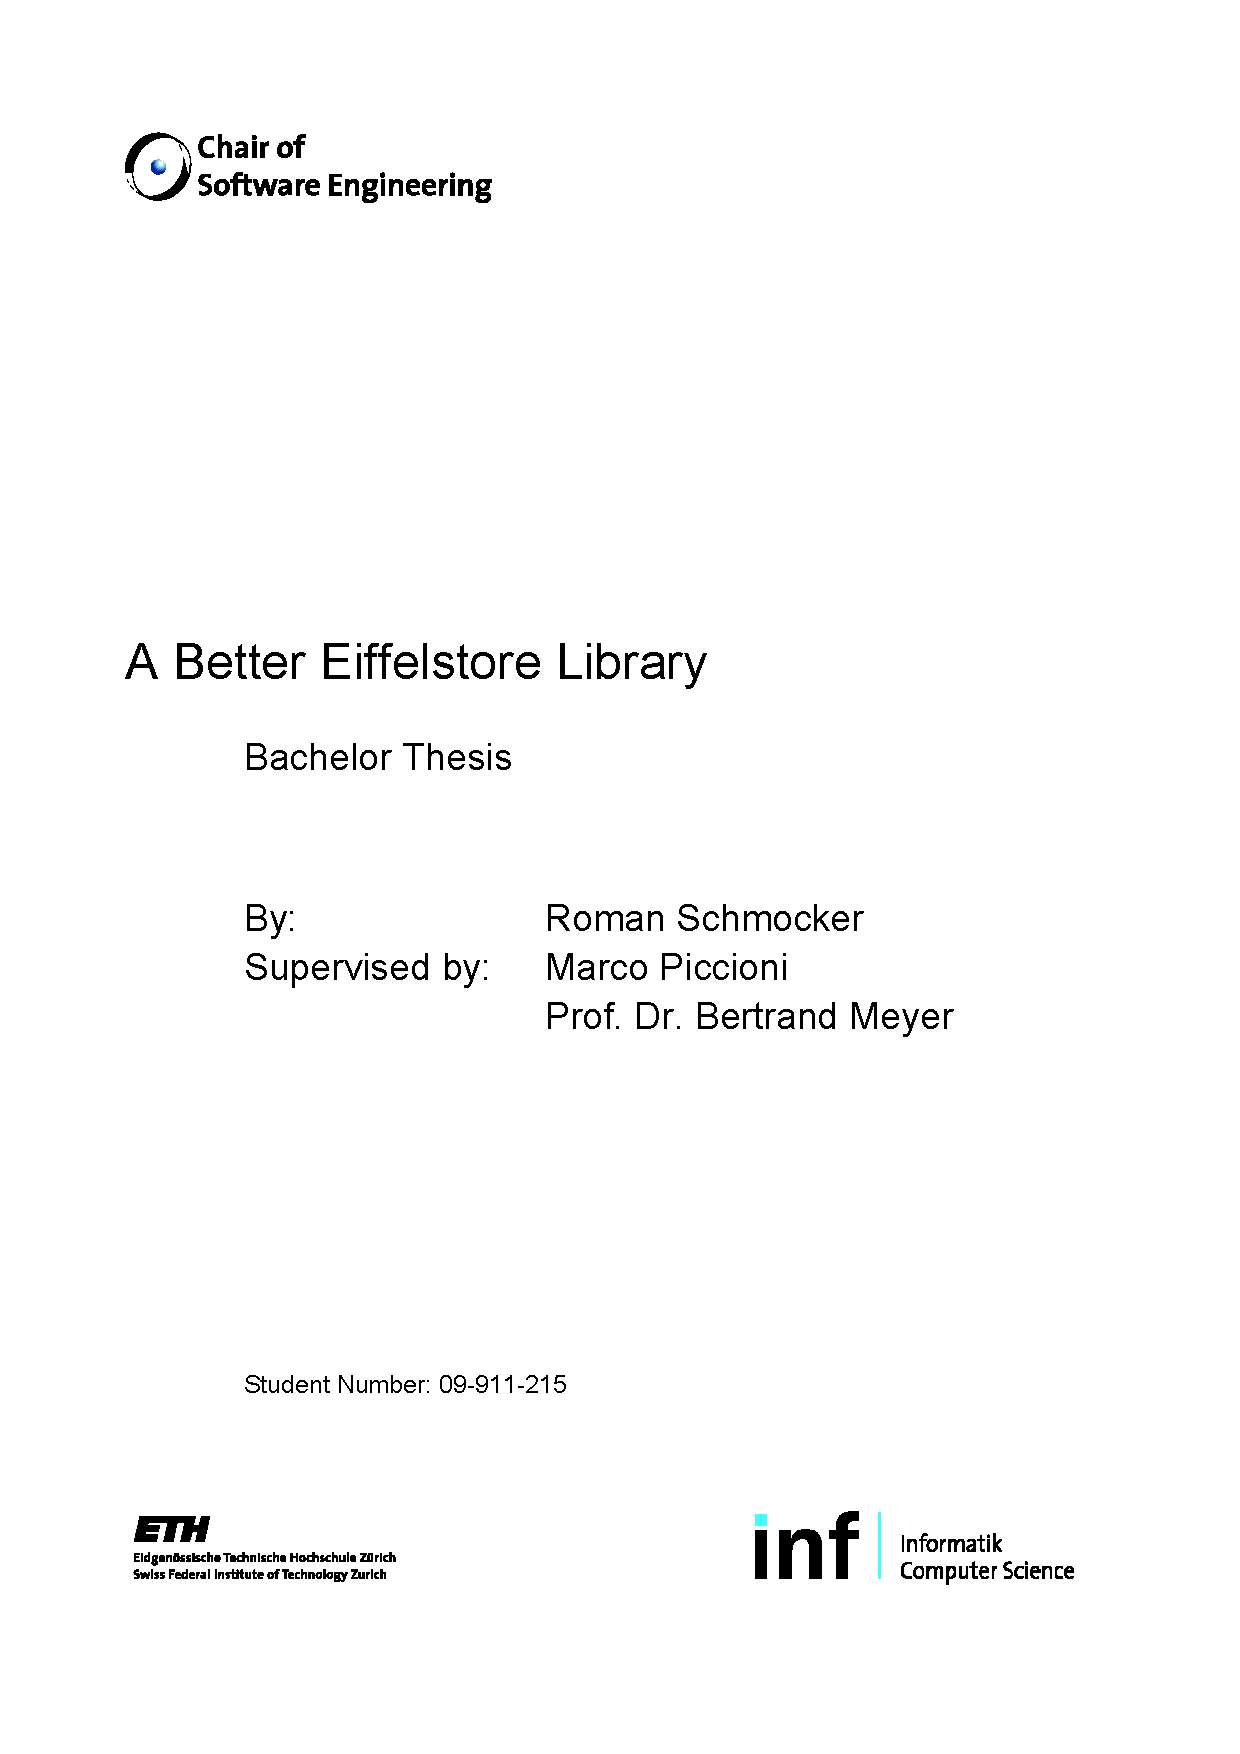
\includepdf {title_page}
%\maketitle

\blankpage

\section*{Abstract}

ABEL is an approach to wrap every existing persistence library under a simple and yet powerful API.
The programming interface of ABEL is completely transparent to the actual storage mechanism, and it supports the CRUD operations, transactions, and some advanced features like result filtering based on some criteria.

ABEL has a flexible framework that allows to adapt the API to basically any existing persistence solution.
The framework has a reusable object-relational mapper at its core and is open for extensions and customization.

\blankpage

\tableofcontents

\chapter{Introduction}
\pagenumbering{arabic}


\section{Introduction}

The Eiffel language \cite{EcmaEiffel} \cite{Meyer09} features a lot of different persistence libraries, and every solution has its own advantages and drawback.
A database such as MySQL \cite {MySQL} for example is quite fast, but it comes at the expence of the object-relational impedance mismatch.\cite{ORImpedance}
A serialization library on the other hand is easier to handle for the programmer, but its performance rapidly decreases for large data sets.

It is very hard to switch from one persistence solution to another, because all have their own interface.
Even changing for example the database from MySQL to Oracle \cite{Oracle} is usually very hard to achieve, if only because their SQL dialects are different.

To overcome such problems we have developed a new library called ABEL, which is the acronym for ``A better Eiffelstore library''.
ABEL tries to unify existing persistence libraries unter a simple and yet powerful API, which is completely transparent to the actual storage mechanism.


\section{Overview}
This thesis is basically splitted into two parts: The API tutorial and the technical documentation.

In the first part you will be introduced to the basic operations of the API, like the CRUD (Create, Read, Update, Delete) operations or transaction handling.

The second part is an introduction to the general architecture of ABEL and some selected topics like the object-relational mapping layer or the main interfaces for backend abstraction.

\chapter{API tutorial}


\section{Getting started}

\subsection{The setup}
In this little tutorial, we are using PERSON objects to show the usage of the API.
In the source code below you will see that ABEL handles objects "as they are", meaning that you don't need to inherit from any specific class to make them persistent.

\begin{lstlisting}[language=OOSC2Eiffel, captionpos=b, caption={The PERSON class}, label={lst:person_class}]
class PERSON

create
	make

feature {NONE} -- Initialization

	make (first, last: STRING)
			-- Create a new person
		do
			first_name := first
			last_name := last
			age:= 0
		end

feature -- Basic operations

	celebrate_birthday
			-- Increase age by 1
		do
			age:= age+1
		end

feature -- Access

	first_name: STRING
		-- First name of person
	last_name: STRING
		-- Last name of person

	age: INTEGER
		-- The person's age

end

\end{lstlisting}




There are 3 very important classes in ABEL:
\begin{itemize}
 \item The CRUD\_EXECUTOR is, as the name suggests, responsible to execute CRUD commands.
	It is the core interface in ABEL and completely transparent to the actual storage backend.

 \item The OBJECT\_QUERY [G] class is used to describe a read operation in ABEL. 
	You can execute such a query in the CRUD\_EXECUTOR. 
	The result will be objects of type G.

 \item The deferred class REPOSITORY provides an abstraction to the actual storage mechanism.
	Every CRUD\_EXECUTOR is attached to a specific REPOSITORY.
\end{itemize}

\subsection{Initialization}

To start using the library, we therefore first need to create a REPOSITORY.
For this tutorial we will use a simple IN\_MEMORY\_REPOSITORY, which simulates a relational database but stores all values in memory.
Although this repository will not give us any persistence, we use it here because initialization is very easy.


\begin{lstlisting}[language=OOSC2Eiffel, captionpos=b, caption={The TUTORIAL class}, label={lst:tutorial_class}]
class TUTORIAL

create
	make

feature {NONE} -- Initialization

	make
		-- Set up a simple in-memory repository
		local
			repository:PS_IN_MEMORY_REPOSITORY
		do
			create repository.make
			create executor.make (repository)
		end

feature
	
	executor: PS_CRUD_EXECUTOR
		-- The CRUD executor used throughout the tutorial

end
\end{lstlisting}

We will use this class throughout the tutorial. You can assume that listings of Eiffel features are inside the TUTORIAL class, if they are not enclosed in another class declaration.

If you want to set up ABEL using a real persistence mechanism, you can read section ~\ref{section:advanced_initialization}, ``Advanced Initialization.''

\section{Basic operations}

\subsection{Query}

A query for objects is done by creating a OBJECT\_QUERY [G] object and executing it in the CRUD\_EXECUTOR.
The generic parameter G of the OBJECT\_QUERY instance denotes the type of objects that should be queried.
%In this tutorial they are objects of type PERSON, but ABEL will also return all objects that are descendants of type PERSON.

After a successful execution of the query, you can get the result through the iteration cursor OBJECT\_QUERY.result\_cursor.
Having an iteration cursor as a result has several advantages, e.g. support for lazy loading or the across syntax\todo{cite?}, as you will see in the next example:

\begin{lstlisting}[language=OOSC2Eiffel, captionpos=b, caption={}, label={lst:simple_query}]
	simple_query: LINKED_LIST [PERSON]
		-- Query all person objects from the current repository
		local
			query:PS_OBJECT_QUERY[PERSON]
		do
			create Result.make
			create query.make
			executor.execute_query (query)

			across query as	query_result
			loop
				Result.extend (query_result.item)
			end
		end
\end{lstlisting}

Usually the result of such a query is very big, and you are probably only interested in objects that meet a certain criteria, e.g. all persons of age 20.
ABEL has a mechanism to support this kind of result filtering. You can read about it in section ~\ref{sec:query}.

Please note that ABEL does not enforce any kind of order on a query result.

\begin{comment}
ABEL can also filter the query results in advance so you only get a result set that meets certain criteria: 

\begin{lstlisting}[language=OOSC2Eiffel, captionpos=b, caption={}, label={lst:simple_filtered_query}]
	simple_filtered_query (name:STRING; age:INTEGER): detachable PERSON
		-- Query a person object from the current repository
		local
			query:PS_OBJECT_QUERY[PERSON]
			criterion:PS_PREDEFINED_CRITERION
		do
			create query.make
			create criterion.make ("last_name", "=", name)
			query.set_criterion (criterion)

			from
				executor.execute_query (query)
			until 
				query.result_cursor.after
			loop
				if query.result_cursor.item.age = age then 
					Result:= query.result_cursor.item
				end
			end
		end
\end{lstlisting}

This is just a very simple example for a query with a certain criterion.
ABEL has a powerful mechanism that also supports a logical combinations of multiple criteria, or using agents for filtering.
You can read more about criteria in section XY.

\end{comment}

\subsection{Insert and update}

Inserting and updating an object is done through CRUD\_EXECUTOR.insert (or CRUD\_EXECUTOR.update, respectively): 

\begin{lstlisting}[language=OOSC2Eiffel, captionpos=b, caption={}, label={lst:simple_insert}]
	simple_insert_and_update (a_person:PERSON)
		-- insert `a_person' into the current repository
		do
			executor.insert (a_person)
			a_person.celebrate_birthday
			executor.update (a_person)
		end
\end{lstlisting}


\subsection{Deletion}
\label{subsection:simple_delete}

Deletion is done through the CRUD\_EXECUTOR.delete feature, like shown in the following example:

\begin{lstlisting}[language=OOSC2Eiffel, captionpos=b, caption={}, label={lst:simple_delete}]
	delete_person (name:STRING)
		-- Delete the person called `name'.
		local
			query: PS_OBJECT_QUERY[PERSON]
		do
			-- First retrieve the person from the database
			create query.make
			executor.execute_query (query)
			across query as query_result
			loop
				if query_result.item.last_name.equals (name) then

					-- Now delete him
					executor.delete (query_result.item)
				end
			end
		end
\end{lstlisting}

There is another way to delete objects which uses a query and some matching criteria. 
You can read about it in section ~\ref{subsection:deletion_query}.

\subsection{Recognizing Objects}
\label{subsection:recognize_objects}

ABEL keeps track of objects that have been inserted or queried.
This is important because in case of an update or delete, ABEL needs to internally map the object in the current execution of the program to its specific entry in the database.
Because of that, you can't update or delete an object that is not yet known to ABEL.
As an example, the following two functions will fail:

\begin{lstlisting}[language=OOSC2Eiffel, captionpos=b, caption={}, label={lst:failing_update_delete}]
	failing_update
		-- Try and fail to update a new person object
		local
			a_person:PERSON
		do
			create a_person.make ("Albo", "Bitossi")
			executor.update (a_person)
				-- Results in a precondition violation
		end

	failing_delete (name:STRING)
		-- Try and fail to delete a new person object
		local
			a_person:PERSON
		do
			create a_person.make ("Albo", "Bitossi")
			executor.delete (a_person) 
				-- Results in a precondition violation
		end
\end{lstlisting}

Please note that there's another way to delete objects, described in Section ~\ref{subsection:deletion_query}, which doesn't have this restriction.

The CRUD\_EXECUTOR.is\_persistent feature can tell you if a specific object is known to ABEL and therefore has a link to its entry in the data\-base.



%Insert the section about advanced queries here:
\section{Advanced Queries}
\label{sec:query}

\subsection{The query mechanism}

As you already know, queries to the database are done by creating a new \lstinline!OBJECT_QUERY! and letting it be executed by the \lstinline!CRUD_EXECUTOR!.
The generic parameter \lstinline!G! of the \lstinline!OBJECT_QUERY! instance determines the type of the objects that will be returned, including any conforming type (e.g. descendants of \lstinline!G!).

ABEL will by default load an object completely, meaning all objects that can be reached by following references will be loaded as well (see also section ~\ref{sec:references}).


\subsection{Criteria}

You can filter your query results by setting criteria in the query object, using the \lstinline!OBJECT_QUERY.set_criteria! feature.
There are two types of criteria: predefined and agent criteria.

\subsubsection{Predefined Criteria}
Predefined criteria take an attribute name, an operator and a value. 
During a read operation, ABEL checks the attribute value of the freshly retrieved object against the value set in the criterion, and filters objects that don't satisfy the criterion.

Most supported operators are pretty self-describing (see Listing ~\ref{lst:factory_interface}).
The likely exception is the \lstinline!like!-operator, which does pattern-matching on strings.
You can give the \lstinline!like!-operator a pattern as a value which can contain the wildcard characters \lstinline!*! and \lstinline!?!.
The asterisk stands for any number (including zero) of undefined characters, and the question mark means exactly one undefined character.

You can only use attributes that are of a basic type, like strings or numbers, and not every type of attribute supports every operator. 
Valid combinations for each type are:

 \begin{itemize}
  \item Strings: =, like
  \item Any numeric value: $=, <, <=, >, >=$
  \item Booleans: =
 \end{itemize}

Note that for performance reasons it is usually better to use predefined criteria, because they can be compiled to SQL and hence the result can be filtered in the database.

\subsubsection{Agent Criteria}

An agent criterion will filter the objects according to the result of an agent applied to them.

The criterion is initialized with an agent of type \lstinline!PREDICATE [ANY, TUPLE [ANY]]!. 
There should be either an open target or a single open argument, and the type of the objects in the query result should conform to the agent's open operand.


\subsubsection{Creating criteria objects}

The criteria instances are best created using the \lstinline!CRITERION_FACTORY! class.

The main functions of the class are the following: 

\begin{lstlisting}[language=OOSC2Eiffel, captionpos=b, caption={The CRITERION\_FACTORY interface}, label={lst:factory_interface}]
class
	PS_CRITERION_FACTORY
create
	default_create

feature -- Creating a criterion

	new alias "[]" (tuple: TUPLE [ANY]): PS_CRITERION
		-- This function creates a new criterion according to 
		-- the tuple in the argument. The tuple should either 
		-- contain a single PREDICATE or three values with 
		-- type [STRING, STRING, ANY]


	new_agent (a_predicate: PREDICATE [ANY, TUPLE [ANY]]): PS_CRITERION
		-- creates an agent criterion

	new_predefined (object_attribute: STRING; 
		operator: STRING; value: ANY): PS_CRITERION
		-- creates a predefined criterion

feature -- Operators

	equals: STRING = "="

	greater: STRING = ">"

	greater_equal: STRING = ">="

	less: STRING = "<"

	less_equal: STRING = "<="

	like_string: STRING = "like"

end
\end{lstlisting}

To create a new criterion, you basically have two possibilities.
The first one is more traditional, by using \lstinline!CRITERION_FACTORY.new_agent! or \lstinline!CRITERION_FACTORY.new_predefined!.

The second possibility uses some syntactic sugar:
The criterion is created with two brackets after the factory object, of which one is an overloaded operator and the other a tuple definition.
It can be used for both types of criteria, and it is up to you to choose which approach you like best.

\begin{lstlisting}[language=OOSC2Eiffel, captionpos=b, , label={lst:factory_usage}]

	create_criteria_traditional : PS_CRITERION
		-- Create a new criteria using the traditional approach
		do

			-- for predefined criteria
			Result:= 
				factory.new_predefined ("age", factory.less, 5)

			-- for agent criteria
			Result := 
				factory.new_agent (agent age_less_than (?, 5))
		end


	create_criteria_double_bracket : PS_CRITERION
		-- Create a new criteria using the double bracket syntax
		do

			-- for predefined criteria
			Result:= factory[["age", factory.less, 5]]

			-- for agent criteria
			Result := factory[[agent age_less_than (?, 5)]]
		end			


	age_less_than (person: PERSON; age: INTEGER): BOOLEAN
		-- An example agent
		do
			Result:= person.age < age
		end

\end{lstlisting}



\subsubsection{Combining criteria}

If you want to set multiple criterion objects, you can combine them using the standard Eiffel keywords. 
For example, if you want to search for a person called ``Albo Bitossi'' with $age \ne 20$, you can just create a criterion object for each of the constraints and combine them:  

\begin{lstlisting}[language=OOSC2Eiffel, captionpos=b, caption={}, label={lst:search_albo_bitossi}]

	search_albo_bitossi : PS_CRITERION
		-- Create a criterion object that searches for an Albo Bitossi which is not 20 years old
		local
			first_name_criterion:PS_CRITERION
			last_name_criterion: PS_CRITERION
			age_criterion: PS_CRITERION
		do
			first_name_criterion:= 
				factory[[ "first_name", factory.equals, "Albo" ]]

			last_name_criterion := 
				factory[[ "last_name", factory.equals, "Bitossi" ]]

			age_criterion := 
				factory[[ "age", factory.equals, 20 ]]
			
			Result := first_name_criterion and last_name_criterion and not age_criterion

			-- or a bit shorter
			Result := factory[[ "first_name", "=", "Albo" ]] 
				and factory[[ "last_name", "=", "Bitossi" ]] 
				and not factory[[ "age", "=", 20 ]]
		end
\end{lstlisting}

ABEL supports the three standard logical operators \lstinline!AND!, \lstinline!OR! and \lstinline!NOT!. 
Their precedence is the same as in Eiffel, which means that \lstinline!NOT! is stronger than \lstinline!AND!, which in turn is stronger than \lstinline!OR!.


\subsection{Deletion queries}
\label{subsection:deletion_query}


As mentioned previously, there is another way to perform a deletion in the repository.
When you call \lstinline!CRUD_EXECUTOR.execute_deletion_query!, ABEL will delete all objects in the database that would have been retrieved by executing the query normally.
You can look at the following example and compare it with its variation in section ~\ref{subsection:simple_delete}.

\begin{lstlisting}[language=OOSC2Eiffel, captionpos=b, caption={}, label={lst:deletion_query}]
	delete_person (name:STRING)
		-- Delete `name' using a deletion query.
		local
			deletion_query: PS_OBJECT_QUERY[PERSON]
			criterion:PS_PREDEFINED_CRITERION
		do
			create deletion_query.make
			create criterion.make ("last_name", "=", name)
			deletion_query.set_criterion (criterion)
			executor.execute_deletion_query (deletion_query)
		end
\end{lstlisting}

It depends upon the situation if you want to use deletion queries or a direct delete command. 
Usually, a direct command is better if you already have the object in memory, whereas deletion queries are nice to use if the object is not yet loaded from the database.

\subsection{Tuple queries}

So far, we've only looked at queries that return objects. However, in ABEL there is a second option to query data which returns tuples as a result.
Consider an example where you just want to have a list of all last names of persons in the database. 
To load every object of type \lstinline!PERSON! might lead to a very bad performance, especially if there is a big object graph attached to each person object.

To solve this problem, you can instead send a \lstinline!TUPLE_QUERY! to the executor. 
The result is an iteration cursor over a list of tuples in which the attributes of an object are stored. The order of these attributes is the one defined in \lstinline!TUPLE_QUERY.projection!.

\begin{lstlisting}[language=OOSC2Eiffel, captionpos=b, caption={}, label={lst:tuple_query_simple}]
	print_all_last_names
		-- Print the last name of all PERSON objects
		local
			query: PS_TUPLE_QUERY[PERSON]
			last_name_index:INTEGER
			single_result: TUPLE
		do
			create query.make
			-- Find out at which position in the tuple the last_name is returned
			last_name_index:= find_index_of_attribute("last_name")

			from
				executor.execute_tuple_query (query)
			until
				query.result_cursor.after
			loop
				single_result:= query.result_cursor.item
				print (single_result [last_name_index] )
			end			
		end
\end{lstlisting}

\subsubsection{Tuple queries and projections}
By default, a \lstinline!TUPLE_QUERY! will only return attributes which are of a basic type, so no references are followed during a retrieve.
You can change this default by calling \lstinline!TUPLE_QUERY.set_projection!, which expects an array of names of the attributes you would like to have.
If you include an attribute name whose type is not a basic one, ABEL will actually retrieve and build the attribute object, and not just another tuple.

\subsubsection{Tuple queries and criteria}
You are restricted to use predefined criteria in tuple queries, because agent criteria expect an object and not a tuple. 
You can still combine them with logical operators.
It is ok to include a predefined criterion on an attribute that is not present in the projection list - these attributes will be loaded internally to check if the object satisfies the criterion, but then they are discarded for the actual result.

\begin{lstlisting}[language=OOSC2Eiffel, captionpos=b, caption={}, label={lst:tuple_projection_selection}]
	print_last_names_of_20_year_old
		-- Print the last name of all PERSON objects with age=20
		local
			query: PS_TUPLE_QUERY[PERSON]
		do
			create query.make

			-- Only return the last_name of persons
			query.set_projection (<<"last_name">>)

			-- Only return persons with age=20
			query.set_criterion (factory [["age", "=", 20]])

			from
				executor.execute_tuple_query (query)
			until
				query.result_cursor.after
			loop
				-- As we only have the last_name in the tuple,
				-- its index has to be 1
				print (query.result_cursor.item [1] )
			end			
		end
\end{lstlisting}



\section{Dealing with references}
\label {sec:references}

In ABEL, a basic type is an object of type STRING, BOOLEAN, CHARACTER or any numeric object like REAL or INTEGER.
The PERSON class has attributes that are of a basic type only, and those are stored together as a single unit in the database.

However, in Eiffel there's also the fact that an object can contain references to other objects.
ABEL is able to handle these references by storing and reconstructing the whole object graph 
(An object graph is sloppily defined as all objects that can be reached by recursively following all references, starting at some root object).

Let's look at the new class CHILD:

\begin{lstlisting}[language=OOSC2Eiffel, captionpos=b, caption={The CHILD class}, label={lst:child_class}]

class 
	CHILD

create
	make

feature {NONE} -- Initialization

	make (first, last: STRING)
			-- Create a new child
		do
			first_name := first
			last_name := last
			age:= 0
		end

feature -- Access

	celebrate_birthday
			-- Increase age by 1
		do
			age:= age+1
		end

feature -- Status report

	first_name: STRING
		-- First name of child
	last_name: STRING
		-- Last name of child

	age: INTEGER
		-- The child's age

feature	-- Parents 

	mother: detachable CHILD
		-- `Current's mother

	father: detachable CHILD
		-- `Current's father
	
	set_mother (a_mother: CHILD)
		-- Set the mother
		do
			mother:= a_mother
		end

	set_father (a_father: CHILD)
		-- Set the father
		do
			father:= a_father
		end
end
\end{lstlisting}


This adds in some complexity: 
Instead of having a single object, ABEL has to insert a CHILD's mother and father as well, and if their parent attribute is attached as well it has to repeat again.
The good news for you is that the examples above will work exactly the same.

However, there are some additional caveats to take into consideration. 
Let's consider a simple example with CHILD objects ``Baby Doe'', ``John Doe'' and ``Grandpa Doe''.
From the name of the object instances you can already guess what the object graph looks like: 

	\begin{center}
\begin{tikzpicture}[->,>=stealth',shorten >=1pt,auto,node distance=6cm,
  thick,main node/.style={rectangle,fill=white,draw}]

  \node[main node] (1) {$Baby Doe$};
  \node[main node] (2) [right of=1] {$John Doe$};
  \node[main node] (3) [right of=2] {$Grandpa Doe$};

 

  \path
    (1) edge node {$father$} (2)
    (2) edge node {$father$} (3);
\end{tikzpicture}
	\end{center}

Now if you insert ``Baby Doe'' into the repository, ABEL will by default follow all references and insert every single object along the object graph, which means that ``John Doe'' and ``Grandpa Doe'' will be inserted as well.
This is usually the desired behaviour, as objects are stored completely that way, but it also has some side effects:

\begin{itemize}
\item Assume an insert of ``Baby Doe'' has happened to an empty database. 
If you now query the database for CHILD objects, it will return exactly the same object graph as above, but the query result will actually have three items, as the object graph consists of three single CHILD objects.
	
\item After you've inserted ``Baby Doe'', it has no effect if you insert ``John Doe'' or ``Grandpa Doe'' afterwards, because they have already been inserted through the first statement.
\end{itemize}

\subsection{Updates}

By default, ABEL does not follow references on updates. So for example the following statement has no effect on the database.

\begin{lstlisting}[language=OOSC2Eiffel, captionpos=b, caption={}, label={lst:reference_update}]
	celebrate_fathers_birthday (a_child: CHILD)
		-- Increase age of `a_child's father
		require
			child_persistent: executor.is_persistent (a_child)
		do
			a_child.father.celebrate_birthday

			-- This won't have any effect
			executor.update (a_child)

			-- however, it works that way
			executor.update (a_child.father)
		end
\end{lstlisting}

\subsection{Going deeper}

ABEL has no limits regarding the depth of an object graph, and it will detect and handle reference cycles correctly. 
You are welcome to test ABEL's capability with very complex objects, however please keep in mind that this will cause a big performance impact.

To overcome this problem, you can either use simple object structures, or you can tell ABEL to only load or store an object up to a certain depth.
You can see how this is done in Section ~\ref{subsection:obect_graph_settings} in the technical documentation, where the whole concept of an object graphs and its depth is described more detailed.



\section{Advanced Initialization}
\label{section:advanced_initialization}

The in-memory repository we've used so far doesn't store data permanently.
This is acceptable for testing or a tutorial, but not in a real application.
Therefore, ABEL ships with repositories for a MySQL database and an SQLite database.

To use them, you currently have to assemble the parts that are needed.
For MySQL, you need to create a MYSQL\_DATABASE and MYSQL\_STRINGS object.
You need them to create the GENERIC\_LAYOUT\_SQL\_BACKEND, which you need in turn to create the RELATIONAL\_REPOSITORY.

The following little factory class show the process for either a MySQL or an SQLite \cite{SQLite} database:

\begin{lstlisting}[language=OOSC2Eiffel, captionpos=b, caption={}, label={lst:advanced_initialization}]

class 
	REPOSITORY_FACTORY

feature -- Connection details
	
	username:STRING = "tutorial"
	password:STRING = "tutorial"

	db_name:STRING = "tutorial"
	db_host:STRING = "127.0.0.1"
	db_port:INTEGER = 3306

	sqlite_filename: STRING = "tutorial.db"

feature -- Factory methods

	create_mysql_repository: PS_RELATIONAL_REPOSITORY
		-- Create a MySQL repository
		local
			database: PS_MYSQL_DATABASE
			mysql_strings: PS_MYSQL_STRINGS
			backend: PS_GENERIC_LAYOUT_SQL_BACKEND
		do
			create database.make (username, password, db_name, db_host, db_port)
			create mysql_strings
			create backend.make (database, strings)
			create Result.make (backend)
		end

	create_sqlite_repository: PS_RELATIONAL_REPOSITORY
		-- Create an SQLite repository
		local
			database: PS_SQLITE_DATABASE
			sqlite_strings: PS_SQLITE_STRINGS
			backend: PS_GENERIC_LAYOUT_SQL_BACKEND
		do
			create database.make (sqlite_filename)
			create sqlite_strings
			create backend.make (database, strings)
			create Result.make (backend)
		end
end	

\end{lstlisting}


That's all. You can now use the repository to create a CRUD\_EXECUTOR and start programming on it.
All examples from this tutorial work exactly the same, no matter if you use the IN\_MEMORY\_REPOSITORY or any of the database repositories.


\section{Transaction handling}

Every CRUD operation in ABEL is executed within a transaction. 
Transactions are created and commited implicitly, which has the advantage that - especially when dealing with complex object graphs - an object doesn't get ``halfway inserted'' in case of an error.

As a user, you also have the possibility to use transactions explicitly. 
This is done by manually creating an object of type TRANSACTION and using the *\_within\_transaction features in CRUD\_EXECUTOR, instead of the normal ones.
For convenience, there is a factory method for transactions built into the executor.

Let's consider an example where you want to update the age of every person by one:

\begin{lstlisting}[language=OOSC2Eiffel, captionpos=b, caption={}, label={lst:update_all_ages}]
	update_ages
		-- Increase everyone's age by one
		local
			query: PS_OBJECT_QUERY[PERSON]
			transaction: PS_TRANSACTION
		do
			create query.make
			transaction := executor.new_transaction

			executor.execute_query_within_transaction (query, transaction)

			across query as query_result
			loop
				query_result.item.celebrate_birthday
				executor.update_within_transaction 
					(query_result.item, transaction)
			end

			transaction.commit

			-- It might be that the transaction has encountered an error at commit time:
			if transaction.has_error then
				print ("Commit has not been successful")
			end
		end
\end{lstlisting}

You can see here as well that a commit may fail, e.g. when a write conflict happened in the database.
The errors are reported in the TRANSACTION.has\_error attribute.
In case of an error, all changes of the transaction are rolled back automatically.

You can also abort a transaction manually by calling TRANSACTION.rollback. 

\subsection{Transaction isolation levels}

ABEL supports the four standard transaction isolation levels found in most database systems:
\begin{itemize}
 \item Read Uncommitted
 \item Read Committed
 \item Repeatable Read
 \item Serializable
\end{itemize}

The different levels are defined in the ``enum class'' TRANSACTION\_\-ISOLATION\_LEVEL.

You can set a transaction isolation level using the feature REPOSITO\-RY.set\_\-transaction\_isolation\_level.
The default transaction isolation level of ABEL is defined by the actual storage backend.

Please note: Not every backend supports all isolation levels.
Therefore a backend can also use a higher isolation level than you actually instruct it to use, but it is not allowed to use a lesser isolation level.



\section{Error handling}

As ABEL is dealing with IO and databases, runtime errors may happen. 
ABEL will in general raise exceptions in case of an error and expose the error to the library user as an ERROR object.
ABEL distinguishes between two different kinds of errors.

\begin{itemize}

\item Fatal errors: Irrecoverable errors happening in a scenario like a broken connection or an integrity constraint violation in the database.
The usual measure is to rollback the current transaction and raise an exception. 
If you catch the exception in a rescue clause and manage to resolve the problem, you can continue using ABEL.

\item Resolvable failures: Those are not really visible to the user, because no exception is raised when they occur.
A typical example is a conflict between two transactions.
ABEL will detect the failure and, in case of implicit transaction management, retry.

If you use explicit transaction management, it will just doom the current transaction to fail at commit time.
\end{itemize}

ABEL represents errors as objects, and all specific error classes inherit from the deferred class ERROR.
The following list shows all errors that can happen at runtime.

If not explicitly stated otherwise, the errors in this lists belong to the first category (Fatal errors).

\begin{itemize}
\item CONNECTION\_PROBLEM: A broken internet link, or a deleted serialization file.
\item TRANSACTION\_CONFLICT: A write conflict between two transactions. This is a resolvable failure.
\item UNRESOLVABLE\_TRANSACTION\_CONFLICT: A conflict in implicit transaction management that doesn't resolve even after a retry
\item ACCESS\_RIGHT\_VIOLATION: Insufficient privileges in database, or no write permission to serialization file.
\item INTERNAL\_ERROR: Any error happening inside the library, like a failed SQL compilation.
\item GENERAL\_ERROR: Anything that doesn't fit into one of the categories above.
\end{itemize}

Please note that this list isn't complete yet. ABEL first needs to get in a releasable state.

If you want to handle an error, you have to add a rescue clause somewhere in your code. 
You can get the actual error from the CRUD\_EXECU\-TOR.error or TRANSACTION.error feature or - as ERROR inherits from DEVELOPER\_EXCEPTION -
by performing an object test on Eiffel's EXCEPTION\_MANAGER.last\_exception.

For your convenience, there is a visitor pattern for all ABEL error types. 
You can just implement the appropriate functions and use it for your error handling code.

The following code shows an example. 
Note that there's some pseudocode inside, and only important features are shown:

\begin{lstlisting}[language=OOSC2Eiffel, captionpos=b, caption={}, label={lst:error_visitor_example}]

class
	MY_PRIVATE_VISITOR
inherit
	PS_ERROR_VISITOR

feature
	shall_retry: BOOLEAN
		-- Should my client retry the operation?

	visit_access_right_violation (
		error: PS_ACCESS_RIGHT_VIOLATION)
		-- Visit an access right violation error
		do
			add_some_privileges
			shall_retry:=True
		end

	visit_connection_problem (error: PS_CONNECTION_PROBLEM)
		-- Visit a connection problem error
		do
			notify_user_of_abort
			shall_retry:=False
		end
end


class
	TUTORIAL

feature

	my_visitor: MY_PRIVATE_VISITOR
		-- A user-defined visitor to react to an error

	executor: PS_CRUD_EXECUTOR
		-- The CRUD executor used throughout the tutorial

	do_something_with_error_handling
		-- Perform some operations. Deal with errors in case of a problem
		do
			-- Some complicated operations
		rescue
			my_visitor.visit (executor.error)
			if my_visitor.shall_retry then
				retry
			else
				-- The exception propagates upwards, and maybe
				-- another feature can handle it
			end
		end
end

\end{lstlisting}





\chapter{Technical documentation}
\section{Limitations of the library}
TODO

Current limitations:
\begin{itemize}
\item Not all features available if adapted to a custom DB layout 
\item Inheritance currently not properly supported (due to limitation of INTERNAL)
\item Reals have rounding error
\item No ordering support (at least not yet)
\item
\end{itemize}

%What exactly has to be here? Is a missing feature (like ordering support) a limitation as well?

\section{Object graph settings}

TODO

%\section{ PART 2: Technical Documentation}

%\subsection{Moved to technical documentation}
%about criteria
%It will internally build a tree of criteria, with specialized AND, OR or NOT instances as nodes and the usual predefined or agent instances as leafs.


%\subsubsection{Performance remarks}

%ABEL will try to let the backend do as much of the filtering as is possible, to reduce the overhead of e.g. network communication or building unnecessary objects.
%This especially means that ABEL will compile predefined queries to SQL if you have a relational database as a backend. 
%However, if there is an agent criterion OR-ed to a predefined criterion, the test can not be made in the database because you might get false negatives.
%Therefore, to have optimal performance, you should consider the following points:

%\begin{itemize}
%\item Try not to use agent criteria if you have a relational database backend.
%\item Try not to use OR on agent criteria.
%\item Try to keep OR-ed agent criteria as deep down the tree as possible (as the above OR-node defaults to true and thus is not checked for in the backend)
%\end{itemize}


\chapter{Conclusions}
\section{Conclusions}

In this thesis, we have developed a software library to access different persitence mechanism.
The library features a simple yet powerful programming interface, which is completely agnostic of the actual backend.

Below the API we developed a very flexible framework to adapt ABEL to a lot of existing storage engines.
The framework includes a reusable object-relational mapping layer, a database library wrapper, and some interfaces for extension and customization.

Based on this framework we have developed an in-memory backend which is useful for testing, and a test suite that is mostly independent of the actual backend.

Furthermore, we have developed a backend that uses a generic data\-base layout for storing objects, working both for MySQL and SQLite data\-bases.

\section{Current limitations}

\begin{itemize}
\item Due to a limitation in \lstinline!INTERNAL! the framework is not able to get ancestors or descendants of a class.
It therefore treats all classes as if they are flat, meaning that all inherited features are defined directly inside the class.
That way ABEL can handle classes inside an inheritance hierarchy, but the drawback of this approach is that a query to objects of class \lstinline!G! will not return descendants of \lstinline!G!.
\item If you adapt ABEL to a custom database layout, it can only handle object types that have corresponding tables in the database.
\item If a custom database layout isn't well designed, e.g. if there are redundancies, you might get into trouble when trying to adapt ABEL to it.
\item Some basic types are not fully supported:
\begin{itemize}
	\item \lstinline!REAL! has a rounding error.
	\item \lstinline!STRING_32! is converted to \lstinline!STRING_8!, which may distort them sometimes.
	\item \lstinline!CHARACTER! is converted to \lstinline!INTEGER! for storage.
	This is usually fine, but in custom database layouts it results in a type mismatch.
\end{itemize}
\item The generic database layout backend doesn't support \lstinline!SPECIAL! yet (or collections in general).
\item The library completely lacks any performance optimization.
\item The retrieval operation in the object-relational mapping layer doesn't support the depth parameter.
\item The error representation is not complete.
\end{itemize}

\section{Future work}
\begin{description}
 \item [Ordering] At the moment, a query result has no defined order. A mechanism to enforce an order in the result set might be useful.
 \item [Update Query] With the current API you can only do an update if the object has been retrieved or inserted before. 
To select the object to be updated, you could also use a \lstinline!QUERY! object, but additionally you need some mechanism to be able to say which attributes should be updated with a new value.
 \item [Performance] Currently there is no optimization in ABEL, and there is a lot that can be done in this area:
 \begin{itemize}
  \item Compile \lstinline!PREDEFINED_CRITERIA! to SQL in order to get smaller results from the database.
 \item Add support for lazy loading in the generic database layout implementation by using SQL cursors instead of normal SELECT statements.
 \item Use prepared statements and maybe even stored procedures instead of normal SQL statements.
 \item Optimize ABEL by trying to reduce network round trip times to a minimum.
 \item Finding and fixing performance bottlenecks in the code with the help of a profiler
\end{itemize}

 \item [Adaptor Framework] Adaption to a specific layout is a tedious task at the moment, as everything has to be hardcoded. 
It would be much easier if you could just define a mapping from classes to tables and attribute names to column names, and the framework takes care of the rest.
As an extension this mapping could be defined in an XML file.
\item [Backends] Extend ABEL to support more backends, e.g.
\begin{itemize}
 \item A serialization library
 \item An object database like db4o
 \item EiffelStore
 \item A NoSQL database like CouchDB
\end{itemize}
 \item [Inheritance] ABEL needs proper inheritance support as soon as the required features in \lstinline!INTERNAL! get implemented.
\item [Transaction management] Some backends, e.g. the in-memory backend or the serialization library, don't support transactions.
 Therefore it would be nice to implement an extension that provides local transaction management by using multiversion concurrency control at the \lstinline!BACKEND_STRATEGY! level.
\item [ESCHER] At the moment, there is an initial integration of ESCHER into the ABEL framework, but the functionality is limited to a simple version check and error reporting in case of a mismatch.
 This solution could be extended to support automatic conversion as well.
\end{description}


{{{
\bibliographystyle {plain}
\bibliography {./references}
}}}
\end{document}